\documentclass[aspectratio=169,10pt]{beamer}

% -------------------------------------------------------
% KAUST Academy Template  --  Python Pathway · Course 1
% -------------------------------------------------------

\usepackage[T1]{fontenc}
\usepackage[utf8]{inputenc}
\usepackage{tikz}
\usetikzlibrary{arrows.meta,positioning,shadows.blur,calc,fit,
                decorations.pathreplacing,shapes.geometric}
\usepackage{array}
\usepackage{tabularx}
\usepackage{booktabs}
\usepackage[most]{tcolorbox}
\usepackage{ragged2e}
\usepackage{adjustbox}
\usepackage{xcolor}
\usepackage{listings}
\usepackage{graphicx}
\usepackage{subcaption}
\usepackage{amsmath,amssymb}
\usepackage{multirow}
\usepackage{multicol}
\usepackage{hyperref}
\hypersetup{colorlinks=true}

% -------------------------------------------------------
% KAUST Stanford Beamer Theme
% (beamerthemeStanford.sty, beamercolorthemestanford.sty,
%  beamerouterthemesimplefooter.sty must be on the TeX path
%  or in the same directory as this file)
% -------------------------------------------------------
\usetheme{Stanford}

\logo{%
  
\includegraphics[height=0.3in]{style_files/kaust_academy_logo.png}\hspace{0.06in}%
  
\includegraphics[height=0.3in]{style_files/LMHLogo_crest.png}%
}

\makeatletter
\let\@@magyar@captionfix\relax
\makeatother

\setbeamertemplate{itemize items}[default]
\setbeamertemplate{itemize subitem}[circle]
\setbeamertemplate{caption}[numbered]
\setbeamertemplate{navigation symbols}{}

% -------------------------------------------------------
% Color Palette  (PrimaryBlue = KAUST Blue RGB 0,51,102)
% -------------------------------------------------------
\definecolor{PrimaryBlue}{RGB}{0,51,102}
\definecolor{LightGray}{RGB}{245,247,250}
\definecolor{LineGray}{RGB}{180,180,180}
\definecolor{CodeGreen}{RGB}{0,118,83}
\definecolor{CodeRed}{RGB}{190,30,30}
\definecolor{CodeBlue}{RGB}{0,55,130}
\definecolor{CodePurple}{RGB}{114,47,145}

% -------------------------------------------------------
% Custom Commands
% -------------------------------------------------------
\newcommand{\blueball}{%
  \tikz[baseline=-0.6ex]\shade[ball color=PrimaryBlue] (0,0) circle (0.065cm);%
}
\setbeamertemplate{itemize item}{\blueball}
\setbeamertemplate{itemize subitem}{\blueball}
\setlength{\leftmargini}{1.1cm}
\setlength{\leftmarginii}{0.8cm}

\newcommand{\keyword}[1]{\textcolor{PrimaryBlue}{\textbf{#1}}}
\newcommand{\myitem}[1]{\item #1\vspace{0.04cm}}

% Numbered-circle helper
\newcommand{\numcircle}[1]{%
  \tikz[baseline=-0.7ex]\node[circle,shade,ball color=PrimaryBlue,
    text=white,font=\scriptsize\bfseries,inner sep=1.2pt,
    minimum size=0.18cm]{#1};%
}
\newenvironment{numberedlines}%
  {\begin{tabular}{@{}p{0.42cm}p{\dimexpr\textwidth-0.75cm\relax}@{}}}%
  {\end{tabular}}
\newcommand{\nline}[2]{\numcircle{#1} & #2 \\[0.13cm]}

% Placeholder badge (for notebook-covered slides)
\newcommand{\placeholderbadge}{%
  \begin{tikzpicture}[remember picture,overlay]
    \node[anchor=north east,fill=orange!18,draw=orange!70!black,
          rounded corners=1mm,inner xsep=2mm,inner ysep=0.8mm,
          font=\scriptsize\bfseries,text=orange!55!black]
      at ([xshift=-0.28cm,yshift=-1.0cm]current page.north east)
      {PLACEHOLDER --- notebook will cover this};
  \end{tikzpicture}%
}

% -------------------------------------------------------
% tcolorbox Styles
% -------------------------------------------------------
\tcbset{
  lecturebox/.style={
    enhanced,
    colback=LightGray,
    colframe=LineGray,
    boxrule=0.35pt,
    arc=2mm,
    left=1.6mm,right=1.6mm,top=0.8mm,bottom=0.8mm,
    drop shadow={black!45!white,opacity=0.35,
                 shadow xshift=1.2mm,shadow yshift=-1.2mm},
    fonttitle=\normalsize,
    coltitle=white,
    colbacktitle=PrimaryBlue,
    boxed title style={arc=2mm,boxrule=0pt},
    attach boxed title to top left={xshift=0mm,yshift=-0.5mm},
    boxed title size=title,
  },
  plainbox/.style={
    enhanced,
    colback=LightGray,
    colframe=LineGray,
    boxrule=0.35pt,
    arc=2mm,
    left=1.6mm,right=1.6mm,top=0.8mm,bottom=0.8mm,
  }
}

% -------------------------------------------------------
% Python / Code Listing Styles
% -------------------------------------------------------
\lstdefinestyle{pycode}{
  language=Python,
  basicstyle=\ttfamily\scriptsize,
  columns=fullflexible,keepspaces=true,showstringspaces=false,
  breaklines=true,frame=single,rulecolor=\color{LineGray},
  backgroundcolor=\color{gray!6},
  keywordstyle=\color{CodeBlue}\bfseries,
  stringstyle=\color{CodeRed},
  commentstyle=\color{CodeGreen},
  xleftmargin=0pt,xrightmargin=0pt
}
\lstdefinestyle{pycodesmall}{style=pycode,basicstyle=\ttfamily\tiny}
\lstdefinestyle{pycodelarge}{language=Python,
  basicstyle=\ttfamily\large,columns=fullflexible,
  keepspaces=true,showstringspaces=false,frame=single,
  rulecolor=\color{LineGray},backgroundcolor=\color{gray!6},
  keywordstyle=\color{CodeBlue}\bfseries,
  stringstyle=\color{CodeRed},commentstyle=\color{CodeGreen},
  xleftmargin=0pt,xrightmargin=0pt}
\lstdefinestyle{pycodemedium}{language=Python,
  basicstyle=\ttfamily\normalsize,columns=fullflexible,
  keepspaces=true,showstringspaces=false,frame=single,
  rulecolor=\color{LineGray},backgroundcolor=\color{gray!6},
  keywordstyle=\color{CodeBlue}\bfseries,
  stringstyle=\color{CodeRed},commentstyle=\color{CodeGreen},
  xleftmargin=0pt,xrightmargin=0pt}
\lstdefinestyle{termcode}{basicstyle=\ttfamily\large,
  columns=fullflexible,keepspaces=true,showstringspaces=false,
  frame=single,rulecolor=\color{LineGray},backgroundcolor=\color{gray!6}}
\lstdefinestyle{outcode}{basicstyle=\ttfamily\large,
  columns=fullflexible,keepspaces=true,showstringspaces=false,
  frame=single,rulecolor=\color{LineGray},backgroundcolor=\color{gray!6}}
\lstdefinestyle{pseudo}{basicstyle=\ttfamily\large,
  columns=fullflexible,keepspaces=true,showstringspaces=false,
  frame=single,rulecolor=\color{LineGray},backgroundcolor=\color{gray!6},
  xleftmargin=0pt,xrightmargin=0pt}
\lstdefinestyle{pseudocode}{basicstyle=\ttfamily\large,
  columns=fullflexible,keepspaces=true,showstringspaces=false,
  frame=single,rulecolor=\color{LineGray},backgroundcolor=\color{gray!6}}

% -------------------------------------------------------
% TikZ Diagram Styles
% -------------------------------------------------------
\tikzset{
  flowbox/.style={draw=black!85,rounded corners=2mm,fill=LightGray,
    minimum width=2.15cm,minimum height=0.68cm,align=center,font=\normalsize},
  flowarrow/.style={-{Latex[length=2.5mm,width=2.0mm]},
    line width=0.8pt,draw=PrimaryBlue},
  levelbox/.style={draw=black!70,rounded corners=2mm,fill=LightGray,
    text width=3.65cm,minimum height=1.15cm,align=center,font=\normalsize},
  codebox/.style={draw=black!70,rounded corners=2mm,fill=gray!7,
    text width=3.3cm,minimum height=1.1cm,align=center,font=\normalsize},
  terminator/.style={draw,rounded corners=2.5mm,minimum width=2.4cm,
    minimum height=0.48cm,fill=gray!5,align=center},
  process/.style={draw,rectangle,minimum width=2.3cm,
    minimum height=0.52cm,fill=gray!5,align=center},
  decision/.style={draw,diamond,aspect=2.05,inner sep=1.3pt,
    minimum width=2.75cm,minimum height=1.1cm,fill=gray!5,align=center},
  io/.style={draw,trapezium,trapezium left angle=70,
    trapezium right angle=110,minimum width=2.4cm,
    minimum height=0.55cm,fill=gray!5,align=center},
}

% -------------------------------------------------------
% Presentation Metadata
% -------------------------------------------------------
\title[Intermediate Python]{Intermediate Python}
% \subtitle{AI Specialization $\cdot$ Python Pathway}
\author[KAUST Academy]{%
  \begin{tabular}{c}
    \Large Naeemullah Khan
  \end{tabular}
  \vspace{-3ex}%
}
\institute{%
  \vskip 8pt
  \begin{figure}
    \centering
    
\includegraphics[height=0.5in]{style_files/kaust_logo.png}\qquad
    
\includegraphics[height=0.5in]{style_files/LMHLogo.png}
  \end{figure}
  \vskip 6pt
  KAUST Academy\\[3pt]
  King Abdullah University of Science and Technology\\[3pt]
  Stage~1 $\cdot$ Course~2%
}
\date{\today}

% =====================================================

% -------------------------------------------------------
% Course 2 extra commands
% -------------------------------------------------------
\newcommand{\codeword}[1]{\texttt{#1}}
\newcommand{\code}[1]{\texttt{#1}}
\newcommand{\blue}[1]{\textcolor{PrimaryBlue}{\textbf{#1}}}
\newenvironment{bluebox}[1]{%
  \vspace{0.08cm}\begin{tcolorbox}[lecturebox,title={#1},fontupper=\small]%
}{\end{tcolorbox}\vspace{0.05cm}}
\lstdefinestyle{py}{language=Python,basicstyle=\ttfamily\scriptsize,
  keywordstyle=\color{CodeBlue}\bfseries,stringstyle=\color{CodeRed},
  commentstyle=\color{CodeGreen},showstringspaces=false,
  backgroundcolor=\color{gray!6},frame=single,framerule=0.3pt,
  rulecolor=\color{LineGray},columns=fullflexible,keepspaces=true,
  breaklines=true}

\begin{document}


% ── COURSE TITLE SLIDE ──────────────────────────────────────────────────────
% ------------------------------------------
% Title / Cover Slide  (footer visible, header suppressed)
% ------------------------------------------
\begin{noheadline}
\begin{frame}
\maketitle
\end{frame}
\end{noheadline}



% ── MODULE 1 TITLE SLIDE ─────────────────────────────────────────────────────
\begin{noheadline}
\begin{frame}
\frametitle{Module 1: FUNCTIONS}
\vspace{1.2cm}
\begin{center}
  {\fontsize{30}{36}\selectfont\textbf{Module 1}}\\[0.35cm]
  {\fontsize{25}{30}\selectfont FUNCTIONS}\\[0.7cm]
  \tcbox[colback=PrimaryBlue!6,colframe=PrimaryBlue,arc=3mm,boxrule=1pt,left=8mm,right=8mm,top=4mm,bottom=4mm,fontupper=\Large]{def, arguments, scope, recursion, and lambda}
\end{center}
\end{frame}
\end{noheadline}


% 2
\begin{frame}[fragile]
\frametitle{Module Content}
\small
This module covers designing reusable, well-documented functions — including scope, recursion, first-class behaviour, and lambda expressions.

\vspace{0.16cm}
\begin{columns}[T,totalwidth=0.96\textwidth]
\begin{column}{0.48\textwidth}
\begin{itemize}\setlength\itemsep{0.08cm}
  \item \keyword{Functions}: using \codeword{def}, function calls, and program flow.
  \item \keyword{Arguments}: positional, keyword, and default parameter values.
  \item \keyword{Return values}: \codeword{return}, \codeword{print}, and side effects.
  \item \keyword{Docstrings}: documenting functions clearly.
\end{itemize}
\end{column}
\begin{column}{0.48\textwidth}
\begin{itemize}\setlength\itemsep{0.08cm}
  \item \keyword{Scope}: the LEGB rule, local/global variables, \codeword{global} and \codeword{nonlocal}.
  \item \keyword{Pure functions} vs.\ side effects.
  \item \keyword{Recursion}: factorial, Fibonacci, and recursive thinking.
  \item \keyword{First-class functions}: passing functions and lambda expressions.
\end{itemize}
\end{column}
\end{columns}
\end{frame}


\begin{frame}[fragile]
\frametitle{Functions as Black Boxes}
\small
A \keyword{function} is a named sequence of instructions. You give it inputs, it performs a task, and it may return a result.

\vspace{0.35cm}
\begin{center}
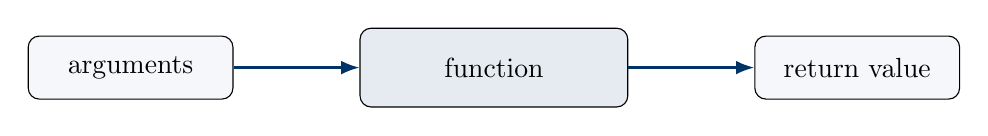
\begin{tikzpicture}[node distance=1.6cm, >=Latex]
  \node[draw,rounded corners,fill=LightGray,minimum width=2.6cm,minimum height=0.8cm] (a) {arguments};
  \node[draw,rounded corners,fill=PrimaryBlue!10,minimum width=3.4cm,minimum height=1.0cm,right=of a] (f) {function};
  \node[draw,rounded corners,fill=LightGray,minimum width=2.6cm,minimum height=0.8cm,right=of f] (r) {return value};
  \draw[->,thick,PrimaryBlue] (a) -- (f);
  \draw[->,thick,PrimaryBlue] (f) -- (r);
\end{tikzpicture}
\end{center}

\vspace{0.15cm}
\begin{lstlisting}[style=pycode]
price = round(6.8275, 2)
print(price)      # 6.83
\end{lstlisting}

\begin{tcolorbox}[lecturebox,title=Key idea]
You do not need to know how \texttt{round()} is implemented. You only need to know what arguments it expects and what result it returns.
\end{tcolorbox}
\end{frame}

\begin{frame}[fragile]
\frametitle{Defining Functions with def}
\small
We define a function with \codeword{def}. The function body is indented, just like \codeword{if} statements and loops.

\vspace{0.2cm}
\begin{lstlisting}[style=pycode]
def cube_volume(side_length):
    volume = side_length ** 3
    return volume

print(cube_volume(2))   # 8
\end{lstlisting}

\begin{tcolorbox}[lecturebox,title=Vocabulary]
\begin{itemize}\setlength\itemsep{0.05cm}
  \item \keyword{Function name}: \texttt{cube\_volume}
  \item \keyword{Parameter}: \texttt{side\_length}, the name used inside the function
  \item \keyword{Argument}: \texttt{2}, the value passed when calling the function
  \item \keyword{return}: sends a result back to the caller
\end{itemize}
\end{tcolorbox}
\end{frame}

\begin{frame}[fragile]
\frametitle{Function Calls and Program Flow}
\small
A function definition is remembered by Python, but the body does not run until the function is called.

\vspace{0.15cm}
\begin{columns}[T,totalwidth=0.96\textwidth]
\begin{column}{0.52\textwidth}
\begin{lstlisting}[style=pycode]
def area(width, height):
    return width * height

room = area(4, 6)
print(room)
\end{lstlisting}
\end{column}
\begin{column}{0.42\textwidth}
\begin{tcolorbox}[lecturebox,title=Execution order]
\begin{enumerate}\small
  \item Python stores the function definition.
  \item Python reaches \texttt{area(4, 6)}.
  \item Parameters receive the arguments.
  \item The function returns \texttt{24}.
  \item The caller stores it in \texttt{room}.
\end{enumerate}
\end{tcolorbox}
\end{column}
\end{columns}
\end{frame}

\begin{frame}[fragile]
\frametitle{Positional vs. Keyword Arguments}
\small
Arguments can be matched by \keyword{position} or by \keyword{name}.

\vspace{0.1cm}
\begin{lstlisting}[style=pycode]
def describe_student(name, major, year):
    return f"{name} studies {major} in year {year}."

# Positional: order matters
print(describe_student("Aisha", "AI", 2))

# Keyword: names make the call clearer
print(describe_student(name="Aisha", major="AI", year=2))
print(describe_student(year=2, name="Aisha", major="AI"))
\end{lstlisting}

\begin{tcolorbox}[lecturebox,title=Beginner habit]
Use keyword arguments when many numbers or similar-looking values are passed. They make code easier to read.
\end{tcolorbox}
\end{frame}

\begin{frame}[fragile]
\frametitle{Default Parameter Values}
\small
A default parameter value is used when the caller does not provide that argument.

\vspace{0.15cm}
\begin{lstlisting}[style=pycode]
def greet(name, language="English"):
    if language == "Arabic":
        return f"Ahlan, {name}!"
    return f"Hello, {name}!"

print(greet("Sara"))                    # uses default
print(greet("Sara", language="Arabic"))
\end{lstlisting}

\begin{tcolorbox}[lecturebox,title=Rule]
Parameters with default values should usually come after parameters without defaults.
\end{tcolorbox}
\end{frame}

\begin{frame}[fragile]
\frametitle{return, print, and Side Effects}
\small
A function can \keyword{return} a value, or it can do something visible such as printing or writing a file.

\vspace{0.1cm}
\begin{columns}[T,totalwidth=0.96\textwidth]
\begin{column}{0.48\textwidth}
\begin{tcolorbox}[lecturebox,title=Returns a value]
\begin{lstlisting}[style=pycode]
def add(a, b):
    return a + b

x = add(2, 3)
\end{lstlisting}
Good for calculations and reuse.
\end{tcolorbox}
\end{column}
\begin{column}{0.48\textwidth}
\begin{tcolorbox}[lecturebox,title=Has a side effect]
\begin{lstlisting}[style=pycode]
def print_total(a, b):
    print(a + b)

print_total(2, 3)
\end{lstlisting}
Good when the task is output.
\end{tcolorbox}
\end{column}
\end{columns}
\end{frame}

\begin{frame}[fragile]
\frametitle{Docstrings: Documenting Functions}
\small
A \keyword{docstring} explains what a function does. It is written as a string immediately under the function header.

\vspace{0.1cm}
\begin{lstlisting}[style=pycode]
def rectangle_area(width, height):
    """Return the area of a rectangle.

    width and height must be non-negative numbers.
    """
    return width * height
\end{lstlisting}

\begin{tcolorbox}[lecturebox,title=Good docstrings answer]
\begin{itemize}\setlength\itemsep{0.05cm}
  \item What does this function do?
  \item What do the parameters mean?
  \item What does it return?
  \item Are there assumptions or special cases?
\end{itemize}
\end{tcolorbox}
\end{frame}

\begin{frame}[fragile]
\frametitle{Variable Scope: The LEGB Rule}
\small
When Python sees a name, it searches for it in a specific order called \keyword{LEGB}.

\vspace{0.10cm}
\begin{center}
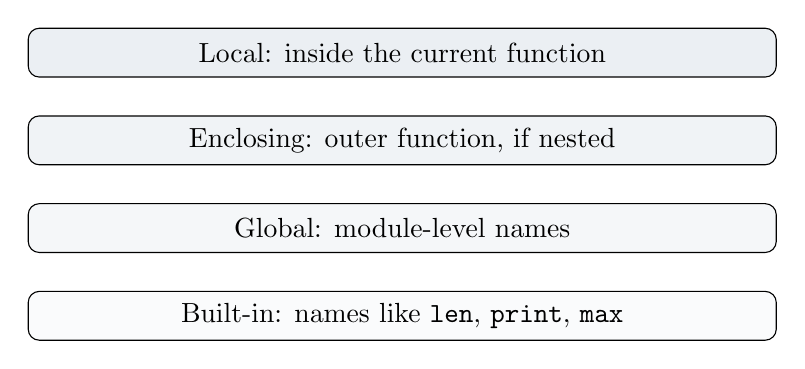
\begin{tikzpicture}[node distance=0.48cm]
\node[draw,rounded corners,fill=PrimaryBlue!8,minimum width=9.5cm,minimum height=0.62cm] (l) {Local: inside the current function};
\node[draw,rounded corners,fill=PrimaryBlue!6,minimum width=9.5cm,minimum height=0.62cm,below=of l] (e) {Enclosing: outer function, if nested};
\node[draw,rounded corners,fill=PrimaryBlue!4,minimum width=9.5cm,minimum height=0.62cm,below=of e] (g) {Global: module-level names};
\node[draw,rounded corners,fill=PrimaryBlue!2,minimum width=9.5cm,minimum height=0.62cm,below=of g] (b) {Built-in: names like \texttt{len}, \texttt{print}, \texttt{max}};
\end{tikzpicture}
\end{center}

\begin{tcolorbox}[lecturebox,title=Key idea]
A variable created inside a function is normally local to that function.
\end{tcolorbox}
\end{frame}

\begin{frame}[fragile]
\frametitle{Local and Global Variables}
\small
A local variable lives inside a function. A global variable is defined outside functions.

\vspace{0.1cm}
\begin{lstlisting}[style=pycode]
message = "global message"

def show_message():
    message = "local message"
    print("Inside:", message)

show_message()
print("Outside:", message)
\end{lstlisting}

\begin{tcolorbox}[lecturebox,title=What happens?]
The local \texttt{message} inside the function does not replace the global \texttt{message}. They are two different variables with the same name in different scopes.
\end{tcolorbox}
\end{frame}

\begin{frame}[fragile]
\frametitle{global and nonlocal}
\small
Use \codeword{global} to update a module-level variable. Use \codeword{nonlocal} to update a variable from an enclosing function.

\vspace{0.1cm}
\begin{columns}[T,totalwidth=0.96\textwidth]
\begin{column}{0.48\textwidth}
\begin{lstlisting}[style=pycodesmall]
count = 0

def increment():
    global count
    count += 1
\end{lstlisting}
\end{column}
\begin{column}{0.48\textwidth}
\begin{lstlisting}[style=pycodesmall]
def make_counter():
    count = 0
    def increment():
        nonlocal count
        count += 1
        return count
    return increment
\end{lstlisting}
\end{column}
\end{columns}

\begin{tcolorbox}[lecturebox,title=Beginner warning]
These keywords are useful, but frequent use can make programs harder to understand. Prefer passing values and returning results when possible.
\end{tcolorbox}
\end{frame}

\begin{frame}[fragile]
\frametitle{Pure Functions vs. Side Effects}
\small
A \keyword{pure function} depends only on its inputs and returns a result without changing the outside world.

\vspace{0.1cm}
\begin{columns}[T,totalwidth=0.96\textwidth]
\begin{column}{0.48\textwidth}
\begin{tcolorbox}[lecturebox,title=Pure function]
\begin{lstlisting}[style=pycodesmall]
def total_price(price, tax):
    return price + price * tax
\end{lstlisting}
Same input gives same output.
\end{tcolorbox}
\end{column}
\begin{column}{0.48\textwidth}
\begin{tcolorbox}[lecturebox,title=Side effect]
\begin{lstlisting}[style=pycodesmall]
items = []

def add_item(item):
    items.append(item)
\end{lstlisting}
Changes something outside itself.
\end{tcolorbox}
\end{column}
\end{columns}
\vspace{0.15cm}
\begin{tcolorbox}[lecturebox,title=Why this matters]
Pure functions are easier to test. Side effects are sometimes necessary, but they should be intentional.
\end{tcolorbox}
\end{frame}

\begin{frame}[fragile]
\frametitle{Recursion: A Function Calling Itself}
\small
\keyword{Recursion} solves a problem by reducing it to a smaller version of the same problem.

\vspace{0.15cm}
\begin{columns}[T,totalwidth=0.96\textwidth]
\begin{column}{0.50\textwidth}
Every recursive function needs:
\begin{itemize}\setlength\itemsep{0.06cm}
  \item a \keyword{base case}: when to stop,
  \item a \keyword{recursive case}: how to make progress,
  \item trust that the smaller call returns the right result.
\end{itemize}
\end{column}
\begin{column}{0.42\textwidth}
\begin{tcolorbox}[lecturebox,title=Call stack idea]
Each function call waits for the smaller call to finish. Python remembers these waiting calls in the \keyword{call stack}.
\end{tcolorbox}
\end{column}
\end{columns}
\end{frame}

\begin{frame}[fragile]
\frametitle{Recursive Example: Factorial}
\small
Factorial means multiplying a number by all positive integers below it.

\vspace{0.1cm}
\begin{lstlisting}[style=pycode]
def factorial(n):
    """Return n! for a non-negative integer n."""
    if n == 0:
        return 1                 # base case
    return n * factorial(n - 1)   # recursive case

print(factorial(5))              # 120
\end{lstlisting}

\begin{tcolorbox}[lecturebox,title=Trace]
\texttt{factorial(5)} becomes \texttt{5 * factorial(4)}, then \texttt{4 * factorial(3)}, and so on until \texttt{factorial(0)} returns \texttt{1}.
\end{tcolorbox}
\end{frame}

\begin{frame}[fragile]
\frametitle{Recursive Example: Fibonacci}
\small
The Fibonacci sequence starts with 0 and 1. Each next value is the sum of the previous two values.

\vspace{0.1cm}
\begin{lstlisting}[style=pycode]
def fibonacci(n):
    if n == 0:
        return 0
    if n == 1:
        return 1
    return fibonacci(n - 1) + fibonacci(n - 2)
\end{lstlisting}

\begin{tcolorbox}[lecturebox,title=Important lesson]
This definition is mathematically clear, but it repeats a lot of work. It is useful for learning recursion, not always for performance.
\end{tcolorbox}
\end{frame}

\begin{frame}[fragile]
\frametitle{Functions Are First-Class Objects}
\small
In Python, functions are values. You can store them in variables, pass them to other functions, and return them.

\vspace{0.1cm}
\begin{lstlisting}[style=pycode]
def shout(text):
    return text.upper()

make_loud = shout
print(make_loud("hello"))
\end{lstlisting}

\begin{tcolorbox}[lecturebox,title=Why this matters]
This idea enables callbacks, sorting keys, decorators, event handlers, and many library patterns.
\end{tcolorbox}
\end{frame}

\begin{frame}[fragile]
\frametitle{Passing Functions as Arguments}
\small
A function that receives another function is called a \keyword{higher-order function}.

\vspace{0.1cm}
\begin{lstlisting}[style=pycode]
def apply_twice(func, value):
    return func(func(value))

def add_one(x):
    return x + 1

print(apply_twice(add_one, 10))   # 12
\end{lstlisting}

\begin{tcolorbox}[lecturebox,title=Concept]
\texttt{apply\_twice} does not know what \texttt{func} does. It only knows it can call it.
\end{tcolorbox}
\end{frame}

\begin{frame}[fragile]
\frametitle{Lambda Expressions}
\small
A \keyword{lambda} is a small anonymous function. Use it for short operations, not large logic.

\vspace{0.1cm}
\begin{lstlisting}[style=pycode]
square = lambda x: x * x
add_tax = lambda price: price * 1.15

print(square(5))
print(add_tax(100))
\end{lstlisting}

\begin{tcolorbox}[lecturebox,title=Rule of thumb]
If a lambda becomes hard to read, write a normal \texttt{def} function instead.
\end{tcolorbox}
\end{frame}

% ── MODULE 2 TITLE SLIDE ─────────────────────────────────────────────────────
\begin{noheadline}
\begin{frame}
\frametitle{Module 2: STRINGS \& TEXT PROCESSING}
\vspace{1.2cm}
\begin{center}
  {\fontsize{30}{36}\selectfont\textbf{Module 2}}\\[0.35cm]
  {\fontsize{25}{30}\selectfont STRINGS \& TEXT PROCESSING}\\[0.7cm]
  \tcbox[colback=PrimaryBlue!6,colframe=PrimaryBlue,arc=3mm,boxrule=1pt,left=8mm,right=8mm,top=4mm,bottom=4mm,fontupper=\Large]{String methods, formatting, and Unicode}
\end{center}
\end{frame}
\end{noheadline}


% ── MODULE 2 CONTENT SLIDE ───────────────────────────────────────────────────
\begin{frame}
\frametitle{Module Content}
\small
This module covers Python's rich set of string tools for text manipulation, formatting, and Unicode support.

\vspace{0.16cm}
\begin{columns}[T,totalwidth=0.96\textwidth]
\begin{column}{0.48\textwidth}
\begin{itemize}\setlength\itemsep{0.08cm}
  \item \keyword{String basics}: text values, quotes, and immutability.
  \item \keyword{Common string methods}: upper, lower, strip, replace, find, and more.
  \item \keyword{Splitting and joining}: tokenizing text and reassembling sequences.
\end{itemize}
\end{column}
\begin{column}{0.48\textwidth}
\begin{itemize}\setlength\itemsep{0.08cm}
  \item \keyword{String formatting}: using \codeword{.format()} for dynamic output.
  \item \keyword{Unicode}: multilingual text support and character encoding.
\end{itemize}
\end{column}
\end{columns}
\end{frame}


\begin{frame}[fragile]
\frametitle{Strings Are Text Values}
\small
A \keyword{string} is a sequence of characters surrounded by quotes.

\vspace{0.2cm}
\begin{lstlisting}[style=pycode]
name = "Aisha"
course = 'Python'
message = "Welcome to Module 3"
\end{lstlisting}

\begin{tcolorbox}[lecturebox,title=Key idea]
Strings can store words, sentences, symbols, numbers written as text, Arabic text, emojis, file names, and user input.
\end{tcolorbox}

\vspace{0.15cm}
\begin{columns}[T,totalwidth=0.96\textwidth]
\begin{column}{0.48\textwidth}
\begin{tcolorbox}[lecturebox,title=String indexing]
\begin{lstlisting}[style=pycodesmall]
word = "Python"
print(word[0])   # P
print(word[1])   # y
\end{lstlisting}
\end{tcolorbox}
\end{column}
\begin{column}{0.48\textwidth}
\begin{tcolorbox}[lecturebox,title=String length]
\begin{lstlisting}[style=pycodesmall]
word = "Python"
print(len(word)) # 6
\end{lstlisting}
\end{tcolorbox}
\end{column}
\end{columns}
\end{frame}

\begin{frame}[fragile]
\frametitle{String Immutability}
\small
Strings are \keyword{immutable}: after a string is created, its characters cannot be changed in place.

\vspace{0.15cm}
\begin{columns}[T,totalwidth=0.96\textwidth]
\begin{column}{0.48\textwidth}
\begin{tcolorbox}[lecturebox,title=This does not work]
\begin{lstlisting}[style=pycodesmall]
word = "Python"
word[0] = "J"      # TypeError
\end{lstlisting}
\end{tcolorbox}
\end{column}
\begin{column}{0.48\textwidth}
\begin{tcolorbox}[lecturebox,title=Create a new string]
\begin{lstlisting}[style=pycodesmall]
word = "Python"
new_word = "J" + word[1:]
print(new_word)    # Jython
\end{lstlisting}
\end{tcolorbox}
\end{column}
\end{columns}

\vspace{0.2cm}
\begin{tcolorbox}[lecturebox,title=Beginner takeaway]
String methods usually \keyword{return a new string}. They do not modify the original string.
\end{tcolorbox}

\begin{lstlisting}[style=pycode]
text = "  python  "
clean = text.strip()
print(text)    # original still has spaces
print(clean)   # new cleaned string
\end{lstlisting}
\end{frame}

\begin{frame}[fragile]
\frametitle{Common String Methods}
\small
String methods are functions attached to string objects. They help clean and transform text.

\vspace{-0.05cm}
\begin{adjustbox}{max width=0.96\textwidth}
\begin{tabular}{@{}lll@{}}
\toprule
\textbf{Method} & \textbf{Purpose} & \textbf{Example idea} \\
\midrule
\codeword{upper()}, \codeword{lower()} & Change letter case & normalize names or commands \\
\codeword{strip()} & Remove surrounding spaces & clean user input \\
\codeword{split()} & Break text into pieces & words or CSV-like text \\
\codeword{join()} & Combine pieces into text & build a sentence or path \\
\codeword{replace()} & Replace matching text & clean symbols or typos \\
\codeword{find()} & Locate a substring & search inside text \\
\codeword{startswith()}, \codeword{endswith()} & Check prefix/suffix & file names, IDs, URLs \\
\bottomrule
\end{tabular}
\end{adjustbox}

\vspace{0.15cm}
\begin{lstlisting}[style=pycode]
raw = "  Python, AI, Data  "
text = raw.strip().lower()
parts = text.split(",")
print(parts)     # ['python', ' ai', ' data']
\end{lstlisting}

\begin{tcolorbox}[lecturebox,title=Habit]
When processing user input, clean it first: remove spaces, normalize case, then compare or analyze.
\end{tcolorbox}
\end{frame}

\begin{frame}[fragile]
\frametitle{Splitting, Joining, and Tokenization}
\small
\keyword{Tokenization} means breaking text into meaningful pieces called tokens. For beginners, a token is often just a word.

\vspace{0.15cm}
\begin{columns}[T,totalwidth=0.96\textwidth]
\begin{column}{0.49\textwidth}
\begin{tcolorbox}[lecturebox,title=Split text]
\begin{lstlisting}[style=pycodesmall]
sentence = "AI helps science"
words = sentence.split()
print(words)
# ['AI', 'helps', 'science']
\end{lstlisting}
\end{tcolorbox}
\end{column}
\begin{column}{0.49\textwidth}
\begin{tcolorbox}[lecturebox,title=Join text]
\begin{lstlisting}[style=pycodesmall]
words = ["AI", "helps", "science"]
text = " ".join(words)
print(text)
# AI helps science
\end{lstlisting}
\end{tcolorbox}
\end{column}
\end{columns}

\vspace{0.2cm}
\begin{tcolorbox}[lecturebox,title=NLP preview]
Many language-processing tasks begin by cleaning text, splitting it into tokens, and counting or comparing those tokens.
\end{tcolorbox}

\end{frame}

\begin{frame}[fragile]
\frametitle{String Formatting with \texttt{.format()}}
\small
The \keyword{.format()} method places values inside placeholders written as \codeword{\{\}}. It is useful for building clear messages from variables.

\vspace{0.15cm}
\begin{columns}[T,totalwidth=0.96\textwidth]
\begin{column}{0.49\textwidth}
\begin{tcolorbox}[lecturebox,title=Basic placeholders]
\begin{lstlisting}[style=pycodesmall]
name = "Sara"
score = 92
msg = "{} scored {}".format(name, score)
print(msg)
# Sara scored 92
\end{lstlisting}
\end{tcolorbox}
\end{column}
\begin{column}{0.49\textwidth}
\begin{tcolorbox}[lecturebox,title=Number formatting]
\begin{lstlisting}[style=pycodesmall]
price = 19.987
print("Price: {:.2f}".format(price))
# Price: 19.99
\end{lstlisting}
\end{tcolorbox}
\end{column}
\end{columns}

\vspace{0.15cm}
\begin{tcolorbox}[lecturebox,title=Named placeholders]
\begin{lstlisting}[style=pycode]
template = "Hello {student}, welcome to {course}."
print(template.format(student="Ali", course="Python"))
\end{lstlisting}
\end{tcolorbox}

\vspace{-0.05cm}
\textbf{Note:} f-strings are often shorter, but \codeword{.format()} is still common in older code and reusable templates.
\end{frame}

\begin{frame}[fragile]
\frametitle{Unicode and Multilingual Text}
\small
Modern programs must handle accented and multilingual text. Python strings are Unicode text.

\vspace{0.15cm}
\begin{lstlisting}[style=pycode]
text = "Cafe Python"
print(len(text))

encoded = text.encode("utf-8")
decoded = encoded.decode("utf-8")
print(decoded)
\end{lstlisting}

\begin{columns}[T,totalwidth=0.96\textwidth]
\begin{column}{0.48\textwidth}
\begin{tcolorbox}[lecturebox,title=Unicode]
A standard way to represent characters from many writing systems.
\end{tcolorbox}
\end{column}
\begin{column}{0.48\textwidth}
\begin{tcolorbox}[lecturebox,title=UTF-8]
A common encoding that stores Unicode text as bytes in files and networks.
\end{tcolorbox}
\end{column}
\end{columns}

\vspace{0.15cm}
\begin{tcolorbox}[lecturebox,title=Practical habit]
When opening text files, specify the encoding when needed: \codeword{open("file.txt", encoding="utf-8")}.
\end{tcolorbox}
\end{frame}

% ── MODULE 3 TITLE SLIDE ─────────────────────────────────────────────────────
\begin{noheadline}
\begin{frame}
\frametitle{Module 3: COLLECTIONS}
\vspace{1.2cm}
\begin{center}
  {\fontsize{30}{36}\selectfont\textbf{Module 3}}\\[0.35cm]
  {\fontsize{25}{30}\selectfont COLLECTIONS}\\[0.7cm]
  \tcbox[colback=PrimaryBlue!6,colframe=PrimaryBlue,arc=3mm,boxrule=1pt,left=8mm,right=8mm,top=4mm,bottom=4mm,fontupper=\Large]{Lists, tuples, dictionaries, and sets}
\end{center}
\end{frame}
\end{noheadline}


% ── MODULE 3 CONTENT SLIDE ───────────────────────────────────────────────────
\begin{frame}
\frametitle{Module Content}
\small
This module covers Python's four core collection types for organising and managing groups of data.

\vspace{0.16cm}
\begin{columns}[T,totalwidth=0.96\textwidth]
\begin{column}{0.48\textwidth}
\begin{itemize}\setlength\itemsep{0.08cm}
  \item \keyword{Lists}: creation, indexing, slicing, mutation, and common methods.
  \item \keyword{List copying}: shallow vs.\ deep copy.
  \item \keyword{Tuples}: immutable ordered data and use cases.
\end{itemize}
\end{column}
\begin{column}{0.48\textwidth}
\begin{itemize}\setlength\itemsep{0.08cm}
  \item \keyword{Dictionaries}: key-value storage, common methods, and nested dicts.
  \item \keyword{Sets}: unique values and set operations.
  \item \keyword{Choosing}: picking the right data structure for the problem.
\end{itemize}
\end{column}
\end{columns}
\end{frame}


\begin{frame}[fragile]
\frametitle{Why Collections Matter}
\begin{bluebox}{Key idea}
A collection stores many related values under one name, instead of creating many separate variables.
\end{bluebox}
\vspace{0.15cm}
\begin{columns}[T]
\begin{column}{0.48\textwidth}
\begin{lstlisting}[style=py]
score1 = 90
score2 = 85
score3 = 92
\end{lstlisting}
\end{column}
\begin{column}{0.48\textwidth}
\begin{lstlisting}[style=py]
scores = [90, 85, 92]
\end{lstlisting}
\end{column}
\end{columns}
\begin{itemize}
  \item Collections make repeated processing easier.
  \item They work naturally with loops and functions.
  \item Different collections are useful for different tasks.
\end{itemize}
\end{frame}

\begin{frame}[fragile]
\frametitle{Lists: Creation, Indexing, and Slicing}
\begin{lstlisting}[style=py]
grades = [95, 82, 77, 90]

first = grades[0]      # 95
last = grades[-1]      # 90
middle = grades[1:3]   # [82, 77]
\end{lstlisting}
\begin{bluebox}{Beginner rule}
Python indexes start at \code{0}. A slice \code{a:b} starts at \code{a} and stops before \code{b}.
\end{bluebox}
\begin{itemize}
  \item Lists preserve order.
  \item Lists can contain numbers, strings, booleans, and even other lists.
\end{itemize}
\end{frame}

\begin{frame}[fragile]
\frametitle{Lists Are Mutable}
\begin{bluebox}{Mutable means changeable}
A list can be edited after it is created.
\end{bluebox}
\begin{lstlisting}[style=py]
items = ["pen", "book", "bag"]
items[0] = "pencil"
items.append("laptop")

print(items)
# ['pencil', 'book', 'bag', 'laptop']
\end{lstlisting}
\begin{itemize}
  \item This is different from strings, which cannot be changed character by character.
  \item Nested lists can represent tables, grids, or grouped data.
\end{itemize}
\end{frame}

\begin{frame}
\frametitle{Common List Methods}
\small
\renewcommand{\arraystretch}{1.25}
\begin{tabularx}{\linewidth}{>{\bfseries}p{2.6cm}X}
\toprule
Method & Purpose \\
\midrule
\code{append(x)} & Add one item to the end. \\
\code{extend(seq)} & Add many items from another iterable. \\
\code{insert(i,x)} & Insert an item at a position. \\
\code{remove(x)} & Remove the first matching value. \\
\code{pop(i)} & Remove and return an item by index; default is last item. \\
\code{sort()} & Sort the list in place. \\
\code{sorted(seq)} & Return a new sorted list. \\
\code{reverse()} & Reverse the list in place. \\
\code{index(x)} & Find the first position of a value. \\
\code{count(x)} & Count occurrences of a value. \\
\bottomrule
\end{tabularx}
\end{frame}

\begin{frame}[fragile]
\frametitle{List Copying: Shallow vs. Deep Copy}
\begin{lstlisting}[style=py]
a = [[1, 2], [3, 4]]
b = a          # same list object
c = a.copy()   # shallow copy
\end{lstlisting}
\begin{bluebox}{Important distinction}
A shallow copy creates a new outer list, but nested objects may still be shared.
\end{bluebox}
\begin{lstlisting}[style=py]
import copy

d = copy.deepcopy(a)  # copies nested objects too
\end{lstlisting}
\begin{itemize}
  \item Use \code{copy()} or slicing for simple one-level lists.
  \item Use \code{copy.deepcopy()} when nested structures must be fully independent.
\end{itemize}
\end{frame}

\begin{frame}[fragile]
\frametitle{Tuples: Immutable Ordered Data}
\begin{lstlisting}[style=py]
point = (3, 5)
month, day, year = (5, 8, 2026)
\end{lstlisting}
\begin{itemize}
  \item A tuple is like a list, but it cannot be changed after creation.
  \item Use tuples for fixed records: coordinates, dates, RGB colors, function results.
\end{itemize}
\begin{bluebox}{Named tuples}
A named tuple gives names to positions, making tuple data easier to read.
\end{bluebox}
\begin{lstlisting}[style=py]
from collections import namedtuple
Point = namedtuple("Point", ["x", "y"])
p = Point(3, 5)
print(p.x, p.y)
\end{lstlisting}
\end{frame}

\begin{frame}[fragile]
\frametitle{Dictionaries: Key--Value Data}
\begin{bluebox}{Key idea}
A dictionary maps each unique key to a value.
\end{bluebox}
\begin{lstlisting}[style=py]
student = {
    "name": "Aisha",
    "major": "AI",
    "year": 2
}

print(student["name"])
student["year"] = 3
\end{lstlisting}
\begin{itemize}
  \item Keys are used instead of numeric indexes.
  \item Values can be numbers, strings, booleans, or other collections.
\end{itemize}
\end{frame}

\begin{frame}
\frametitle{Common Dictionary Methods}
\small
\renewcommand{\arraystretch}{1.25}
\begin{tabularx}{\linewidth}{>{\bfseries}p{3.0cm}X}
\toprule
Method & Purpose \\
\midrule
\code{get(key, default)} & Safely read a value without raising \code{KeyError}. \\
\code{keys()} & View all keys. \\
\code{values()} & View all values. \\
\code{items()} & View key--value pairs. \\
\code{update(other)} & Add or replace multiple pairs. \\
\code{pop(key)} & Remove a key and return its value. \\
\code{setdefault(k, v)} & Return existing value, or create it if missing. \\
\bottomrule
\end{tabularx}
\begin{bluebox}{Beginner habit}
Use \code{get()} when a key may not exist.
\end{bluebox}
\end{frame}

\begin{frame}[fragile]
\frametitle{Nested Dictionaries and Dict Comprehensions}
\begin{lstlisting}[style=py]
students = {
    "Aisha": {"score": 95, "level": "A"},
    "Omar":  {"score": 88, "level": "B"}
}

print(students["Aisha"]["score"])
\end{lstlisting}
\begin{bluebox}{Dictionary comprehension}
Build a dictionary from a pattern.
\end{bluebox}
\begin{lstlisting}[style=py]
squares = {n: n*n for n in range(1, 6)}
# {1: 1, 2: 4, 3: 9, 4: 16, 5: 25}
\end{lstlisting}
\end{frame}

\begin{frame}[fragile]
\frametitle{Sets: Unique Values and Set Operations}
\begin{lstlisting}[style=py]
colors = {"red", "green", "blue", "red"}
print(colors)   # duplicates are removed
\end{lstlisting}
\small
\renewcommand{\arraystretch}{1.25}
\begin{tabularx}{\linewidth}{>{\bfseries}p{3.4cm}X}
\toprule
Operation & Meaning \\
\midrule
\code{a | b} or \code{a.union(b)} & Union: values in either set. \\
\code{a \& b} or \code{a.intersection(b)} & Intersection: values in both sets. \\
\code{a - b} or \code{a.difference(b)} & Difference: values in \code{a} not in \code{b}. \\
\code{a \^ b} & Symmetric difference: values in exactly one set. \\
\bottomrule
\end{tabularx}
\end{frame}

\begin{frame}
\frametitle{Choosing the Right Data Structure}
\small
\renewcommand{\arraystretch}{1.25}
\begin{tabularx}{\linewidth}{>{\bfseries}p{2.4cm}X X}
\toprule
Structure & Best for & Main trade-off \\
\midrule
List & Ordered sequence, indexing, repeated values & Searching can be slower for large data. \\
Tuple & Fixed ordered record & Cannot be changed. \\
Dictionary & Fast lookup by key & Requires meaningful unique keys. \\
Set & Fast membership testing and unique values & No indexing or guaranteed position-based access. \\
\bottomrule
\end{tabularx}
\begin{bluebox}{Performance intuition}
Use a set or dictionary when you repeatedly ask: ``Is this value present?'' or ``What value belongs to this key?''
\end{bluebox}
\end{frame}

% ── MODULE 4 TITLE SLIDE ─────────────────────────────────────────────────────
\begin{noheadline}
\begin{frame}
\frametitle{Module 4: COMPREHENSIONS \& FUNCTIONAL TOOLS}
\vspace{1.2cm}
\begin{center}
  {\fontsize{30}{36}\selectfont\textbf{Module 4}}\\[0.35cm]
  {\fontsize{22}{28}\selectfont COMPREHENSIONS \& FUNCTIONAL TOOLS}\\[0.7cm]
  \tcbox[colback=PrimaryBlue!6,colframe=PrimaryBlue,arc=3mm,boxrule=1pt,left=8mm,right=8mm,top=4mm,bottom=4mm,fontupper=\Large]{Comprehensions, generators, and functional tools}
\end{center}
\end{frame}
\end{noheadline}


% ── MODULE 4 CONTENT SLIDE ───────────────────────────────────────────────────
\begin{frame}
\frametitle{Module Content}
\small
This module introduces compact, expressive Python patterns using comprehensions, generators, and functional tools.

\vspace{0.16cm}
\begin{columns}[T,totalwidth=0.96\textwidth]
\begin{column}{0.48\textwidth}
\begin{itemize}\setlength\itemsep{0.08cm}
  \item \keyword{Comprehensions}: list, dictionary, set, and generator expressions.
  \item \keyword{Nested comprehensions}: multi-level collection building.
  \item \keyword{Generators}: lazy evaluation with generator expressions.
  \item \keyword{Anti-patterns}: avoiding mutation while iterating.
\end{itemize}
\end{column}
\begin{column}{0.48\textwidth}
\begin{itemize}\setlength\itemsep{0.08cm}
  \item \keyword{Functional tools}: \codeword{map()}, \codeword{filter()}, \codeword{zip()}, \codeword{enumerate()}, and \codeword{sorted(key=...)}.
  \item \keyword{Variable-length arguments}: \codeword{*args} and \codeword{**kwargs}.
  \item \keyword{Functional vs.\ imperative}: choosing the right style.
\end{itemize}
\end{column}
\end{columns}
\end{frame}


\begin{frame}[fragile]
\frametitle{Comprehensions: Compact Collection Building}
\begin{bluebox}{Key idea}
A comprehension builds a collection from an existing sequence using a compact loop-like expression.
\end{bluebox}
\begin{columns}[T]
\begin{column}{0.49\textwidth}
\begin{lstlisting}[style=py]
squares = []
for n in range(6):
    squares.append(n*n)
\end{lstlisting}
\end{column}
\begin{column}{0.49\textwidth}
\begin{lstlisting}[style=py]
squares = [n*n for n in range(6)]
\end{lstlisting}
\end{column}
\end{columns}
\begin{itemize}
  \item Use comprehensions when the transformation is short and readable.
  \item Use a normal loop when the logic needs several steps.
\end{itemize}
\end{frame}

\begin{frame}[fragile]
\frametitle{List Comprehensions: Syntax and Conditions}
\begin{lstlisting}[style=py]
# transform every value
squares = [n*n for n in range(1, 6)]

# keep only some values
evens = [n for n in range(10) if n % 2 == 0]

# transform and filter at the same time
labels = [f"ID-{n}" for n in range(5) if n != 3]
\end{lstlisting}
\begin{bluebox}{Pattern}
\code{[expression for item in iterable if condition]}
\end{bluebox}
\end{frame}

\begin{frame}[fragile]
\frametitle{Nested List Comprehensions}
\begin{bluebox}{Use with care}
Nested comprehensions are compact, but they can become hard to read quickly.
\end{bluebox}
\begin{lstlisting}[style=py]
# all coordinate pairs from 0..2 and 0..1
pairs = [(x, y) for x in range(3) for y in range(2)]
\end{lstlisting}
\begin{itemize}
  \item Read it like nested loops: outer loop first, inner loop second.
  \item If students need to pause and decode it, a normal nested loop may be better.
\end{itemize}
\end{frame}

\begin{frame}[fragile]
\frametitle{Dictionary Comprehensions}
\begin{lstlisting}[style=py]
# number -> square
squares = {n: n*n for n in range(1, 6)}

# word -> length
words = ["AI", "Python", "data"]
lengths = {word: len(word) for word in words}
\end{lstlisting}
\begin{bluebox}{Pattern}
\texttt{\{key\_expression: value\_expression for item in iterable\}}
\end{bluebox}
\begin{itemize}
  \item Useful when each item naturally produces a key and a value.
  \item Keys must be unique; repeated keys overwrite earlier values.
\end{itemize}
\end{frame}

\begin{frame}[fragile]
\frametitle{Set Comprehensions}
\begin{lstlisting}[style=py]
names = ["Aisha", "Omar", "Ali", "Aisha"]
first_letters = {name[0] for name in names}

print(first_letters)
# {'A', 'O'}
\end{lstlisting}
\begin{bluebox}{When useful?}
Use a set comprehension when you want unique results from a transformation.
\end{bluebox}
\end{frame}

\begin{frame}[fragile]
\frametitle{Generator Expressions: Lazy Evaluation}
\begin{bluebox}{Key idea}
A generator expression produces values one at a time instead of building the whole collection immediately.
\end{bluebox}
\begin{lstlisting}[style=py]
total = sum(n*n for n in range(1_000_000))
\end{lstlisting}
\begin{itemize}
  \item This can save memory for large data.
  \item Good for feeding values into functions like \code{sum()}, \code{max()}, or \code{any()}.
  \item Use a list comprehension when you need to store or reuse the full list.
\end{itemize}
\end{frame}

\begin{frame}
\frametitle{Comprehension or Explicit Loop?}
\small
\renewcommand{\arraystretch}{1.25}
\begin{tabularx}{\linewidth}{>{\bfseries}p{4.0cm}X}
\toprule
Use a comprehension when... & Use a loop when... \\
\midrule
The logic is one clear transformation. & The logic needs many steps. \\
The condition is short. & You need debugging prints or intermediate variables. \\
The result is a new collection. & You are changing existing state carefully. \\
It improves readability. & It becomes clever but difficult to understand. \\
\bottomrule
\end{tabularx}
\begin{bluebox}{Main principle}
Readable code is better than compressed code.
\end{bluebox}
\end{frame}

\begin{frame}[fragile]
\frametitle{Anti-Pattern: Modifying a List While Iterating}
\begin{lstlisting}[style=py]
numbers = [1, 2, 3, 4, 5]

# Avoid this pattern
for n in numbers:
    if n % 2 == 0:
        numbers.remove(n)
\end{lstlisting}
\begin{bluebox}{Why it is risky}
Changing a list while looping over it can cause items to be skipped or processed incorrectly.
\end{bluebox}
\begin{lstlisting}[style=py]
# Better: build a new list
numbers = [n for n in numbers if n % 2 != 0]
\end{lstlisting}
\end{frame}

\begin{frame}[fragile]
\frametitle{map(): Applying a Function to Every Element}
\small
\codeword{map()} represents the idea of \keyword{transforming each item} in an iterable using the same function.

\vspace{0.18cm}
\begin{lstlisting}[style=pycode]
numbers = [1, 2, 3, 4]

squares = map(lambda x: x ** 2, numbers)
print(list(squares))   # [1, 4, 9, 16]
\end{lstlisting}

\begin{tcolorbox}[lecturebox,title=Key idea]
Use this pattern when every item should be converted in the same way: numbers to squares, text to uppercase, temperatures to another unit, and so on.
\end{tcolorbox}

\vspace{0.1cm}
\begin{tcolorbox}[lecturebox,title=Beginner note]
A normal \codeword{for} loop is often easier to read at first. Learn the concept before worrying about shorter syntax.
\end{tcolorbox}
\end{frame}

\begin{frame}[fragile]
\frametitle{filter(): Selecting Items by a Condition}
\small
\codeword{filter()} keeps only the items that pass a \keyword{predicate}: a function that returns \codeword{True} or \codeword{False}.

\vspace{0.18cm}
\begin{lstlisting}[style=pycode]
numbers = [3, -2, 0, 8, -5, 10]

positives = filter(lambda x: x > 0, numbers)
print(list(positives))  # [3, 8, 10]
\end{lstlisting}

\begin{columns}[T,totalwidth=0.96\textwidth]
\begin{column}{0.47\textwidth}
\begin{tcolorbox}[lecturebox,title=Predicate]
\codeword{lambda x: x > 0} asks a yes/no question about each item.
\end{tcolorbox}
\end{column}
\begin{column}{0.47\textwidth}
\begin{tcolorbox}[lecturebox,title=Result]
Only items where the answer is \codeword{True} are kept.
\end{tcolorbox}
\end{column}
\end{columns}
\end{frame}

\begin{frame}[fragile]
\frametitle{zip(): Combining Multiple Iterables}
\small
\codeword{zip()} pairs items from multiple iterables by position.

\vspace{0.18cm}
\begin{lstlisting}[style=pycode]
names = ["Aisha", "Omar", "Lina"]
scores = [95, 88, 91]

for name, score in zip(names, scores):
    print(f"{name}: {score}")
\end{lstlisting}

\begin{tcolorbox}[lecturebox,title=What happens?]
The first name is paired with the first score, the second name with the second score, and so on.
\end{tcolorbox}

\vspace{0.10cm}
\begin{tcolorbox}[lecturebox,title=Careful]
If the iterables have different lengths, \codeword{zip()} stops when the shortest one ends.
\end{tcolorbox}
\end{frame}

\begin{frame}[fragile]
\frametitle{enumerate(): Counting While Iterating}
\small
\codeword{enumerate()} gives you both the \keyword{index} and the \keyword{value} while looping.

\vspace{0.18cm}
\begin{lstlisting}[style=pycode]
names = ["Aisha", "Omar", "Lina"]

for index, name in enumerate(names):
    print(index, name)
\end{lstlisting}

\begin{columns}[T,totalwidth=0.96\textwidth]
\begin{column}{0.47\textwidth}
\begin{tcolorbox}[lecturebox,title=Why use it?]
Use it when you need the position of each item without manually creating a counter.
\end{tcolorbox}
\end{column}
\begin{column}{0.47\textwidth}
\begin{tcolorbox}[lecturebox,title=Custom start]
\begin{lstlisting}[style=pycodesmall]
for number, name in enumerate(names, start=1):
    print(number, name)
\end{lstlisting}
\end{tcolorbox}
\end{column}
\end{columns}
\end{frame}

\begin{frame}[fragile]
\frametitle{sorted() with a key Function}
\small
\codeword{sorted()} can use a \keyword{key function} to decide how items should be ordered.

\vspace{0.18cm}
\begin{lstlisting}[style=pycode]
words = ["AI", "programming", "data", "Python"]

print(sorted(words))
print(sorted(words, key=len))
\end{lstlisting}

\begin{tcolorbox}[lecturebox,title=Key idea]
\codeword{key=len} means: sort the words by their length, not alphabetically.
\end{tcolorbox}

\vspace{0.1cm}
\begin{lstlisting}[style=pycode]
students = [("Aisha", 95), ("Omar", 88), ("Lina", 91)]

# Sort by score using a small function
print(sorted(students, key=lambda item: item[1]))
\end{lstlisting}
\end{frame}

\begin{frame}[fragile]
\frametitle{Functional vs. Imperative Style}
\small
Python supports both \keyword{imperative} code and \keyword{functional-style} tools.

\vspace{0.18cm}
\begin{columns}[T,totalwidth=0.96\textwidth]
\begin{column}{0.47\textwidth}
\begin{tcolorbox}[lecturebox,title=Imperative style]
Step-by-step instructions.
\begin{lstlisting}[style=pycodesmall]
result = []
for x in numbers:
    if x > 0:
        result.append(x * 2)
\end{lstlisting}
\end{tcolorbox}
\end{column}
\begin{column}{0.47\textwidth}
\begin{tcolorbox}[lecturebox,title=Functional style]
Transform and filter data with functions.
\begin{lstlisting}[style=pycodesmall]
result = map(lambda x: x * 2,
             filter(lambda x: x > 0, numbers))
result = list(result)
\end{lstlisting}
\end{tcolorbox}
\end{column}
\end{columns}

\vspace{0.15cm}
\begin{tcolorbox}[lecturebox,title=Main principle]
Choose the version that is easiest to read. Compact code is not automatically better code.
\end{tcolorbox}
\end{frame}



\begin{frame}[fragile]
\frametitle{Variable-Length Positional Arguments: \texttt{*args}}
\small
Sometimes a function should accept \keyword{any number of positional arguments}. In Python, the common convention is to collect them using \codeword{*args}.

\vspace{0.18cm}
\begin{columns}[T,totalwidth=0.96\textwidth]
\begin{column}{0.52\textwidth}
\begin{lstlisting}[style=pycode]
def average(*args):
    total = 0
    for value in args:
        total += value
    return total / len(args)

print(average(10, 20, 30))
print(average(5, 8, 12, 15))
\end{lstlisting}
\end{column}
\begin{column}{0.42\textwidth}
\begin{tcolorbox}[lecturebox,title=What happens?]
\begin{itemize}\setlength\itemsep{0.06cm}
  \item \codeword{args} becomes a tuple of the extra positional values.
  \item The function can loop over those values.
  \item Use this when the number of inputs is naturally flexible.
\end{itemize}
\end{tcolorbox}
\end{column}
\end{columns}

\begin{tcolorbox}[lecturebox,title=Beginner warning]
Do not use \codeword{*args} just to avoid clear function design. Named parameters are usually better when the inputs are known.
\end{tcolorbox}
\end{frame}


\begin{frame}[fragile]
\frametitle{Variable-Length Keyword Arguments: \texttt{**kwargs}}
\small
Sometimes a function should accept optional named information. In Python, the common convention is to collect extra keyword arguments using \codeword{**kwargs}.

\vspace{0.18cm}
\begin{columns}[T,totalwidth=0.96\textwidth]
\begin{column}{0.52\textwidth}
\begin{lstlisting}[style=pycode]
def print_profile(**kwargs):
    for name, value in kwargs.items():
        print(name, "=", value)

print_profile(name="Aisha",
              field="AI",
              level="beginner")
\end{lstlisting}
\end{column}
\begin{column}{0.42\textwidth}
\begin{tcolorbox}[lecturebox,title=What happens?]
\begin{itemize}\setlength\itemsep{0.06cm}
  \item \codeword{kwargs} stores extra named arguments.
  \item Each argument has a name and a value.
  \item This is useful for optional settings and configuration.
\end{itemize}
\end{tcolorbox}
\end{column}
\end{columns}

\begin{tcolorbox}[lecturebox,title=How to read it]
\codeword{*args} answers: ``How many positional values?''\quad \codeword{**kwargs} answers: ``Which named options were provided?''
\end{tcolorbox}
\end{frame}

% ── MODULE 5 TITLE SLIDE ─────────────────────────────────────────────────────
\begin{noheadline}
\begin{frame}
\frametitle{Module 5: FILE I/O \& EXCEPTION HANDLING}
\vspace{1.2cm}
\begin{center}
  {\fontsize{30}{36}\selectfont\textbf{Module 5}}\\[0.35cm]
  {\fontsize{25}{30}\selectfont FILE I/O \& EXCEPTION HANDLING}\\[0.7cm]
  \tcbox[colback=PrimaryBlue!6,colframe=PrimaryBlue,arc=3mm,boxrule=1pt,left=8mm,right=8mm,top=4mm,bottom=4mm,fontupper=\Large]{File I/O, exceptions, and error handling}
\end{center}
\end{frame}
\end{noheadline}


% ── MODULE 5 CONTENT SLIDE ───────────────────────────────────────────────────
\begin{frame}
\frametitle{Module Content}
\small
This module covers reading and writing files, and building programs that recover gracefully from runtime errors.

\vspace{0.16cm}
\begin{columns}[T,totalwidth=0.96\textwidth]
\begin{column}{0.48\textwidth}
\begin{itemize}\setlength\itemsep{0.08cm}
  \item \keyword{File I/O}: why it matters and opening files with \codeword{open()}.
  \item \keyword{Reading and writing}: text files, modes, and safe handling with \codeword{with}.
  \item \keyword{Binary files}: images and other non-text data.
\end{itemize}
\end{column}
\begin{column}{0.48\textwidth}
\begin{itemize}\setlength\itemsep{0.08cm}
  \item \keyword{Exceptions}: what they are and the exception hierarchy.
  \item \keyword{Handling errors}: \codeword{try}, \codeword{except}, \codeword{else}, and \codeword{finally}.
  \item \keyword{Raising exceptions}: signalling problems and custom exception classes.
\end{itemize}
\end{column}
\end{columns}
\end{frame}


\begin{frame}[fragile]
\frametitle{Why File I/O Matters}
\small
Until now, many programs used values typed directly into code or entered by the user. Real programs often need to \keyword{store}, \keyword{load}, and \keyword{process} data from files.

\vspace{0.25cm}
\begin{columns}[T,totalwidth=0.96\textwidth]
\begin{column}{0.48\textwidth}
\begin{tcolorbox}[lecturebox,title=Examples of input files]
\begin{itemize}\setlength\itemsep{0.05cm}
  \item grades in a text file
  \item experiment readings
  \item configuration files
  \item logs generated by a system
\end{itemize}
\end{tcolorbox}
\end{column}
\begin{column}{0.48\textwidth}
\begin{tcolorbox}[lecturebox,title=Examples of output files]
\begin{itemize}\setlength\itemsep{0.05cm}
  \item reports
  \item cleaned data
  \item saved results
  \item error logs
\end{itemize}
\end{tcolorbox}
\end{column}
\end{columns}

\vspace{0.2cm}
\begin{tcolorbox}[lecturebox,title=Key idea]
File I/O lets a program communicate with the outside world beyond the screen and keyboard.
\end{tcolorbox}
\end{frame}

\begin{frame}[fragile]
\frametitle{Opening Files with \texttt{open()}}
\small
To work with a file, Python needs a \keyword{file object}. The \codeword{open()} function creates that connection.

\vspace{0.15cm}
\begin{lstlisting}[style=pycode]
infile = open("input.txt", "r")    # read text
outfile = open("output.txt", "w")  # write text
logfile = open("log.txt", "a")     # append text
\end{lstlisting}

\begin{center}
\begin{tabularx}{0.92\textwidth}{>{\bfseries\ttfamily}p{1.6cm}X}
\toprule
Mode & Meaning \\
\midrule
r  & read an existing text file \\
w  & write a text file; replace existing content \\
a  & append new text to the end of a file \\
rb & read binary data, such as images \\
wb & write binary data \\
\bottomrule
\end{tabularx}
\end{center}

\begin{tcolorbox}[lecturebox,title=Important warning]
Opening a file in \codeword{"w"} mode clears the old content if the file already exists.
\end{tcolorbox}
\end{frame}

\begin{frame}[fragile]
\frametitle{Reading from Files}
\small
Python gives several ways to read file content. Choose the method that matches the task.

\vspace{0.15cm}
\begin{columns}[T,totalwidth=0.96\textwidth]
\begin{column}{0.52\textwidth}
\begin{lstlisting}[style=pycode]
file = open("story.txt", "r")

all_text = file.read()       # whole file
one_line = file.readline()   # one line
lines = file.readlines()     # list of lines

file.close()
\end{lstlisting}
\end{column}
\begin{column}{0.44\textwidth}
\begin{tcolorbox}[lecturebox,title=When to use what]
\begin{itemize}\setlength\itemsep{0.08cm}
  \item \codeword{read()}: small file, all content needed.
  \item \codeword{readline()}: process one line at a time.
  \item \codeword{readlines()}: keep all lines as a collection.
\end{itemize}
\end{tcolorbox}
\end{column}
\end{columns}

\vspace{0.1cm}
\begin{tcolorbox}[lecturebox,title=Common pattern]
\begin{lstlisting}[style=pycodesmall]
for line in open("story.txt", "r"):
    print(line.strip())
\end{lstlisting}
\end{tcolorbox}
\end{frame}

\begin{frame}[fragile]
\frametitle{Writing to Files}
\small
Writing stores text so it can be used later by another program, notebook, or person.

\vspace{0.15cm}
\begin{columns}[T,totalwidth=0.96\textwidth]
\begin{column}{0.50\textwidth}
\begin{lstlisting}[style=pycode]
outfile = open("report.txt", "w")

outfile.write("Experiment report\n")
outfile.write("Accuracy: 0.92\n")

outfile.close()
\end{lstlisting}
\end{column}
\begin{column}{0.46\textwidth}
\begin{lstlisting}[style=pycode]
lines = [
    "Aisha\n",
    "Omar\n",
    "Sara\n"
]

outfile = open("names.txt", "w")
outfile.writelines(lines)
outfile.close()
\end{lstlisting}
\end{column}
\end{columns}

\vspace{0.2cm}
\begin{tcolorbox}[lecturebox,title=Checkpoint]
\codeword{write()} does not automatically add a new line. Add \codeword{"\\n"} when you want the next output to appear on a new line.
\end{tcolorbox}
\end{frame}

\begin{frame}[fragile]
\frametitle{The \texttt{with} Statement: Safe File Handling}
\small
A safer way to work with files is to use \codeword{with}. It automatically closes the file when the block finishes.

\vspace{0.15cm}
\begin{lstlisting}[style=pycode]
with open("input.txt", "r") as infile:
    for line in infile:
        print(line.strip())

with open("output.txt", "w") as outfile:
    outfile.write("Done\n")
\end{lstlisting}

\begin{tcolorbox}[lecturebox,title=Why this matters]
\begin{itemize}\setlength\itemsep{0.08cm}
  \item Files are closed even if the code inside the block fails.
  \item The code clearly shows where file access starts and ends.
  \item It avoids forgetting \codeword{close()}.
\end{itemize}
\end{tcolorbox}

\begin{tcolorbox}[lecturebox,title=Beginner rule]
Prefer \codeword{with open(...)} for file handling unless you have a special reason not to.
\end{tcolorbox}
\end{frame}

\begin{frame}[fragile]
\frametitle{Binary Files: Images and Other Non-Text Data}
\small
Not all files are text. Images, audio, PDFs, and compressed files are stored as \keyword{binary data}.

\vspace{0.15cm}
\begin{columns}[T,totalwidth=0.96\textwidth]
\begin{column}{0.52\textwidth}
\begin{lstlisting}[style=pycode]
with open("photo.jpg", "rb") as file:
    data = file.read()

print(type(data))  # bytes
print(len(data))   # number of bytes
\end{lstlisting}
\end{column}
\begin{column}{0.44\textwidth}
\begin{tcolorbox}[lecturebox,title=Text vs. binary]
\begin{itemize}\setlength\itemsep{0.08cm}
  \item Text files store characters.
  \item Binary files store bytes.
  \item Use \codeword{rb} and \codeword{wb} for binary content.
\end{itemize}
\end{tcolorbox}
\end{column}
\end{columns}

\vspace{0.15cm}
\begin{tcolorbox}[lecturebox,title=Beginner warning]
Do not read an image with normal \codeword{"r"} text mode. Use \codeword{"rb"} so Python treats it as bytes.
\end{tcolorbox}
\end{frame}

\begin{frame}[fragile]
\frametitle{What Is an Exception?}
\small
An \keyword{exception} is Python's way of saying: ``Something unusual happened, and normal execution cannot continue here.''

\vspace{0.15cm}
\begin{lstlisting}[style=pycode]
number = int("abc")      # ValueError
result = 10 / 0          # ZeroDivisionError
file = open("x.txt")     # FileNotFoundError if missing
\end{lstlisting}

\begin{tcolorbox}[lecturebox,title=Main idea]
Exceptions separate \keyword{detecting a problem} from \keyword{deciding how to handle it}.
\end{tcolorbox}

\begin{center}
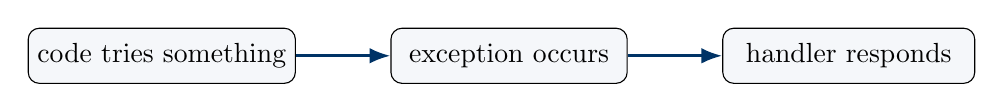
\begin{tikzpicture}[node distance=1.1cm,>=Latex]
\node[draw,rounded corners,fill=LightGray,minimum width=3.1cm,minimum height=0.7cm] (try) {code tries something};
\node[draw,rounded corners,fill=LightGray,right=1.2cm of try,minimum width=3.0cm,minimum height=0.7cm] (err) {exception occurs};
\node[draw,rounded corners,fill=LightGray,right=1.2cm of err,minimum width=3.2cm,minimum height=0.7cm] (handle) {handler responds};
\draw[->,PrimaryBlue,line width=1pt] (try) -- (err);
\draw[->,PrimaryBlue,line width=1pt] (err) -- (handle);
\end{tikzpicture}
\end{center}
\end{frame}

\begin{frame}[fragile]
\frametitle{Exception Hierarchy: The Big Picture}
\small
Python exceptions are organized as classes. For most beginner programs, we catch subclasses of \codeword{Exception}.

\vspace{0.15cm}
\begin{center}
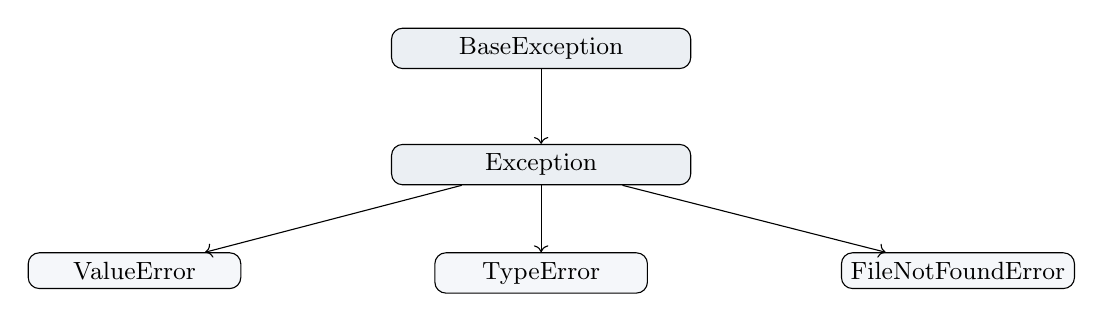
\begin{tikzpicture}[node distance=0.95cm, every node/.style={font=\small}]
\node[draw,rounded corners,fill=PrimaryBlue!8,minimum width=3.8cm] (base) {BaseException};
\node[draw,rounded corners,fill=PrimaryBlue!8,below=of base,minimum width=3.8cm] (exc) {Exception};
\node[draw,rounded corners,fill=LightGray,below left=0.85cm and 1.9cm of exc,minimum width=2.7cm] (value) {ValueError};
\node[draw,rounded corners,fill=LightGray,below=0.85cm of exc,minimum width=2.7cm] (type) {TypeError};
\node[draw,rounded corners,fill=LightGray,below right=0.85cm and 1.9cm of exc,minimum width=2.7cm] (file) {FileNotFoundError};
\draw[->] (base) -- (exc);
\draw[->] (exc) -- (value);
\draw[->] (exc) -- (type);
\draw[->] (exc) -- (file);
\end{tikzpicture}
\end{center}

\begin{tcolorbox}[lecturebox,title=Common examples]
\codeword{ValueError}, \codeword{TypeError}, \codeword{ZeroDivisionError}, \codeword{IndexError}, \codeword{KeyError}, \codeword{FileNotFoundError}, and \codeword{PermissionError}.
\end{tcolorbox}
\end{frame}

\begin{frame}[fragile]
\frametitle{The \texttt{try} and \texttt{except} Blocks}
\small
Put code that might fail inside a \codeword{try} block. Put the recovery plan inside an \codeword{except} block.

\vspace{0.15cm}
\begin{lstlisting}[style=pycode]
try:
    age = int(input("Age: "))
    print("Next year:", age + 1)
except ValueError:
    print("Please enter a whole number.")
\end{lstlisting}

\begin{tcolorbox}[lecturebox,title=How to read it]
\begin{itemize}\setlength\itemsep{0.08cm}
  \item Try to convert the input to an integer.
  \item If conversion fails, handle \codeword{ValueError}.
  \item The program can continue instead of crashing.
\end{itemize}
\end{tcolorbox}
\end{frame}

\begin{frame}[fragile]
\frametitle{Handling File Errors Gracefully}
\small
File operations can fail. The file may not exist, the path may be wrong, or the user may not have permission.

\vspace{0.15cm}
\begin{lstlisting}[style=pycode]
from pathlib import Path

path = Path("data/results.txt")

try:
    text = path.read_text()
    print(text)
except FileNotFoundError:
    print("Could not find the file.")
except PermissionError:
    print("No permission to read this file.")
\end{lstlisting}

\begin{tcolorbox}[lecturebox,title=Key idea]
Good programs do not crash immediately for expected file problems. They explain the problem and give the user a useful message.
\end{tcolorbox}
\end{frame}

\begin{frame}[fragile]
\frametitle{\texttt{else} and \texttt{finally}}
\small
A complete exception structure can include \codeword{else} and \codeword{finally}.

\vspace{0.15cm}
\begin{lstlisting}[style=pycode]
try:
    value = int(input("Number: "))
except ValueError:
    print("Invalid number")
else:
    print("Square:", value ** 2)
finally:
    print("Finished checking input")
\end{lstlisting}

\begin{center}
\begin{tabularx}{0.92\textwidth}{>{\bfseries\ttfamily}p{1.9cm}X}
\toprule
Block & Meaning \\
\midrule
try & code that may raise an exception \\
except & code that handles a specific exception \\
else & runs only if no exception occurred \\
finally & always runs at the end \\
\bottomrule
\end{tabularx}
\end{center}
\end{frame}

\begin{frame}[fragile]
\frametitle{Catch Specific Exceptions}
\small
Avoid catching everything with a bare \codeword{except}. It can hide bugs and make debugging harder.

\vspace{0.15cm}
\begin{columns}[T,totalwidth=0.96\textwidth]
\begin{column}{0.48\textwidth}
\begin{tcolorbox}[lecturebox,title=Better]
\begin{lstlisting}[style=pycodesmall]
try:
    value = int(text)
except ValueError:
    print("Not a number")
\end{lstlisting}
\end{tcolorbox}
\end{column}
\begin{column}{0.48\textwidth}
\begin{tcolorbox}[lecturebox,title=Avoid]
\begin{lstlisting}[style=pycodesmall]
try:
    value = int(text)
except:
    print("Something failed")
\end{lstlisting}
\end{tcolorbox}
\end{column}
\end{columns}

\begin{tcolorbox}[lecturebox,title=Rule of thumb]
Catch the errors you expect and know how to handle. Let unexpected errors show up while you are developing.
\end{tcolorbox}
\end{frame}

\begin{frame}[fragile]
\frametitle{Raising Exceptions}
\small
Sometimes a function detects invalid input and should report the problem to whoever called it.

\vspace{0.15cm}
\begin{lstlisting}[style=pycode]
def withdraw(balance, amount):
    if amount > balance:
        raise ValueError("amount exceeds balance")
    return balance - amount
\end{lstlisting}

\begin{tcolorbox}[lecturebox,title=Re-raising with context]
\begin{lstlisting}[style=pycodesmall]
try:
    amount = float(text)
except ValueError as error:
    raise ValueError("amount must be numeric") from error
\end{lstlisting}
\end{tcolorbox}

\begin{tcolorbox}[lecturebox,title=Key idea]
Use \codeword{raise} when your function cannot continue correctly and the caller should decide what to do.
\end{tcolorbox}
\end{frame}

\begin{frame}[fragile]
\frametitle{Custom Exception Classes}
\small
For larger programs, you can define your own exception type. This makes errors more descriptive.

\vspace{0.15cm}
\begin{lstlisting}[style=pycode]
class InvalidGradeError(Exception):
    pass

def set_grade(grade):
    if grade < 0 or grade > 100:
        raise InvalidGradeError("grade must be between 0 and 100")
    return grade
\end{lstlisting}

\begin{tcolorbox}[lecturebox,title=When useful]
Custom exceptions are useful when your program has domain-specific errors, such as invalid grades, invalid sensor readings, or invalid experiment settings.
\end{tcolorbox}
\end{frame}



\begin{frame}
\frametitle{Thank You}
\vspace{1.75cm}
\begin{center}
{\fontsize{34}{40}\selectfont \textbf{Thank you!}}\\[0.45cm]
{\fontsize{18}{22}\selectfont Questions and discussion}
\end{center}
\vspace{0.80cm}
\begin{tcolorbox}[lecturebox,title=Course takeaway]
Reusable functions, rich data structures, and robust error handling are the building blocks of professional Python programs.
\end{tcolorbox}
\end{frame}


\end{document}
